\subsection{Correction sur la prédiction du modèle sur $w$ entraîné sur le carré}

Dans le but d'améliorer les résultats de Correction obtenus avec $\phi$-FEM, on cherche ici à apprendre la même solution que précédemment mais en entraînant le PINNs sur le carré tout entier (et pas seulement sur $\Omega$ défini par un cercle). 

Dans le cas de l'entraînement sur le cercle, on considère les paramètres par défaut (CONFIG 0) pour le modèle :

\begin{figure}[H]
	\centering
	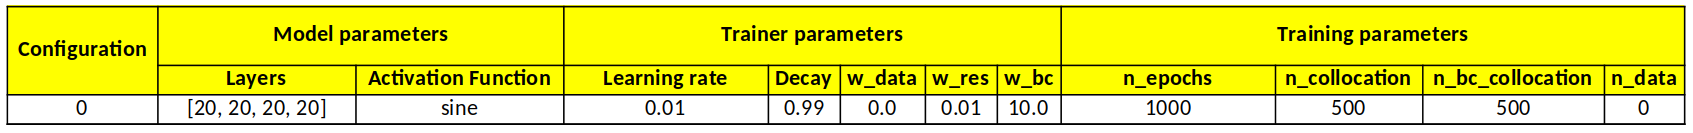
\includegraphics[width=0.8\linewidth]{"train_sur_carre/Cercle_config_0.png"}
	\caption{Paramètres du PINNs (entraînement sur le Cercle).}
\end{figure}

Dans le cas de l'entraînement sur le Carré, on considère les paramètres par défaut sauf pour le nombre de points de collocations (CONFIG 1). On considère en fait plus de points à l'intérieur et sur le bord (car sur le carré les paramètres par défaut n'étaient pas suffisants) :

\begin{figure}[H]
	\centering
	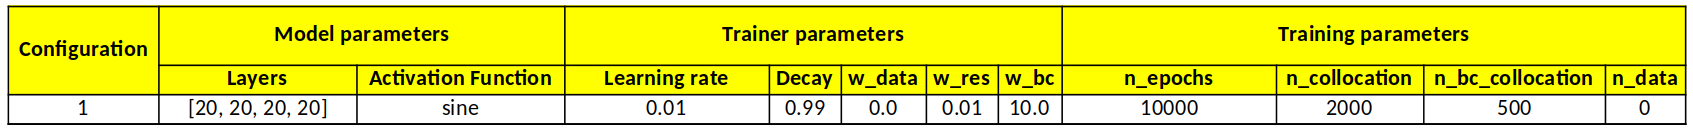
\includegraphics[width=0.8\linewidth]{"train_sur_carre/Carre_config_1.png"}
	\caption{Paramètres du PINNs (entraînement sur le Carré).}
\end{figure}

En entraînant le PINNs à déterminer $u=\phi w$, on obtient les résultats d'entraînement suivant - à gauche : résultat sur le carré / à droite : application d'un masque :

\vspace{-20pt}
\begin{center}
	\begin{minipage}{0.48\linewidth}
		\begin{figure}[H]
			\centering
			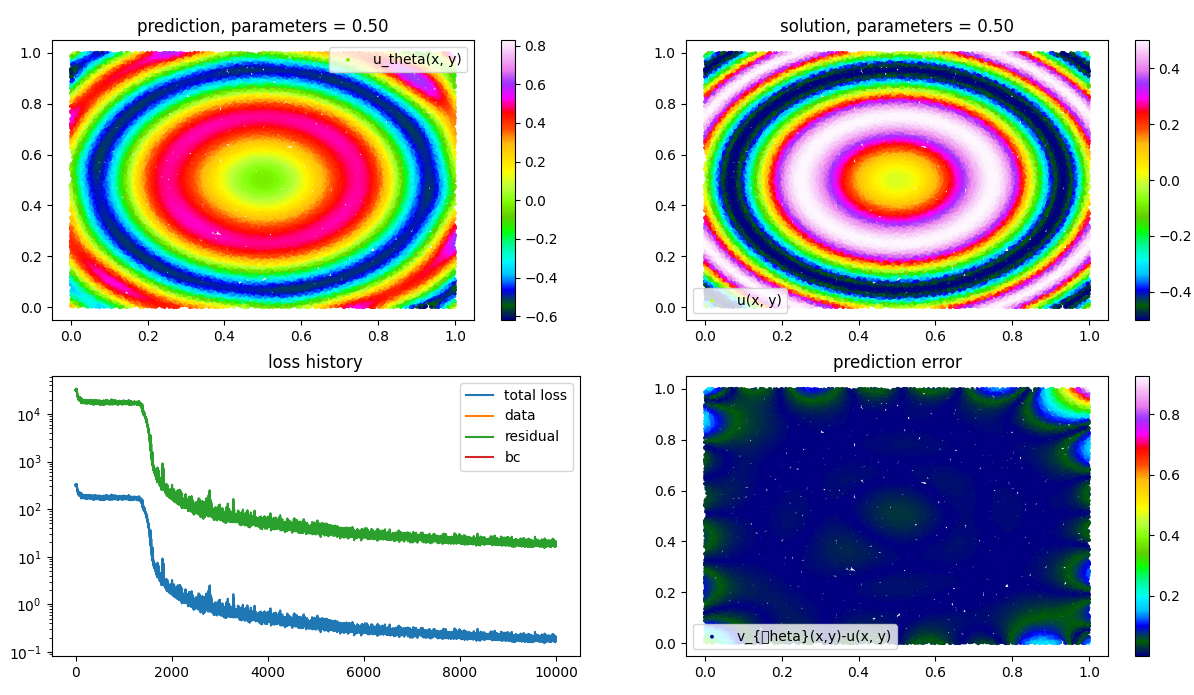
\includegraphics[width=\linewidth]{"train_sur_carre/Carre_model_1_exact_bc.png"}
			\caption{Training $f$ fixé sans le masque.}
		\end{figure}
	\end{minipage}
	\begin{minipage}{0.48\linewidth}
		\begin{figure}[H]
			\centering
			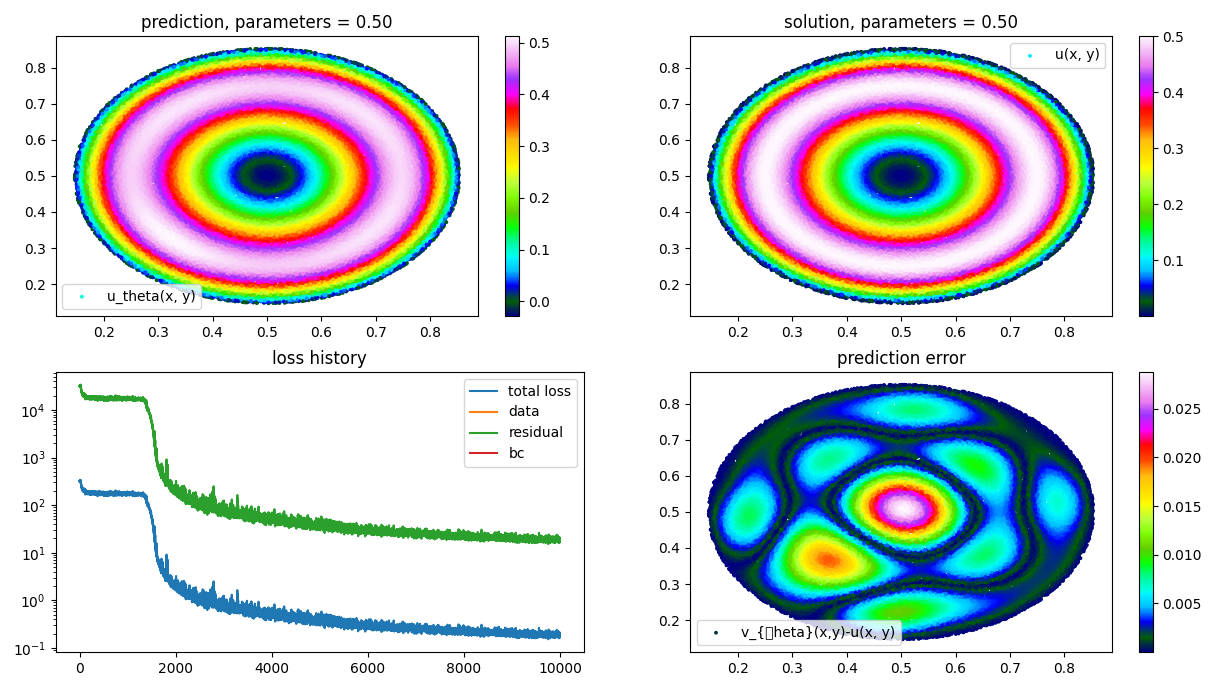
\includegraphics[width=\linewidth]{"train_sur_carre/Carre_model_1_exact_bc_mask.png"}
			\caption{Training $f$ fixé avec le masque.}
		\end{figure}
	\end{minipage}
\end{center}

Pour $S=0.5$, on obtient les résultats suivants pour la correction par addition avec FEM :

\vspace{-20pt}
\begin{center}
	\begin{minipage}{0.48\linewidth}
		\begin{figure}[H]
			\centering
			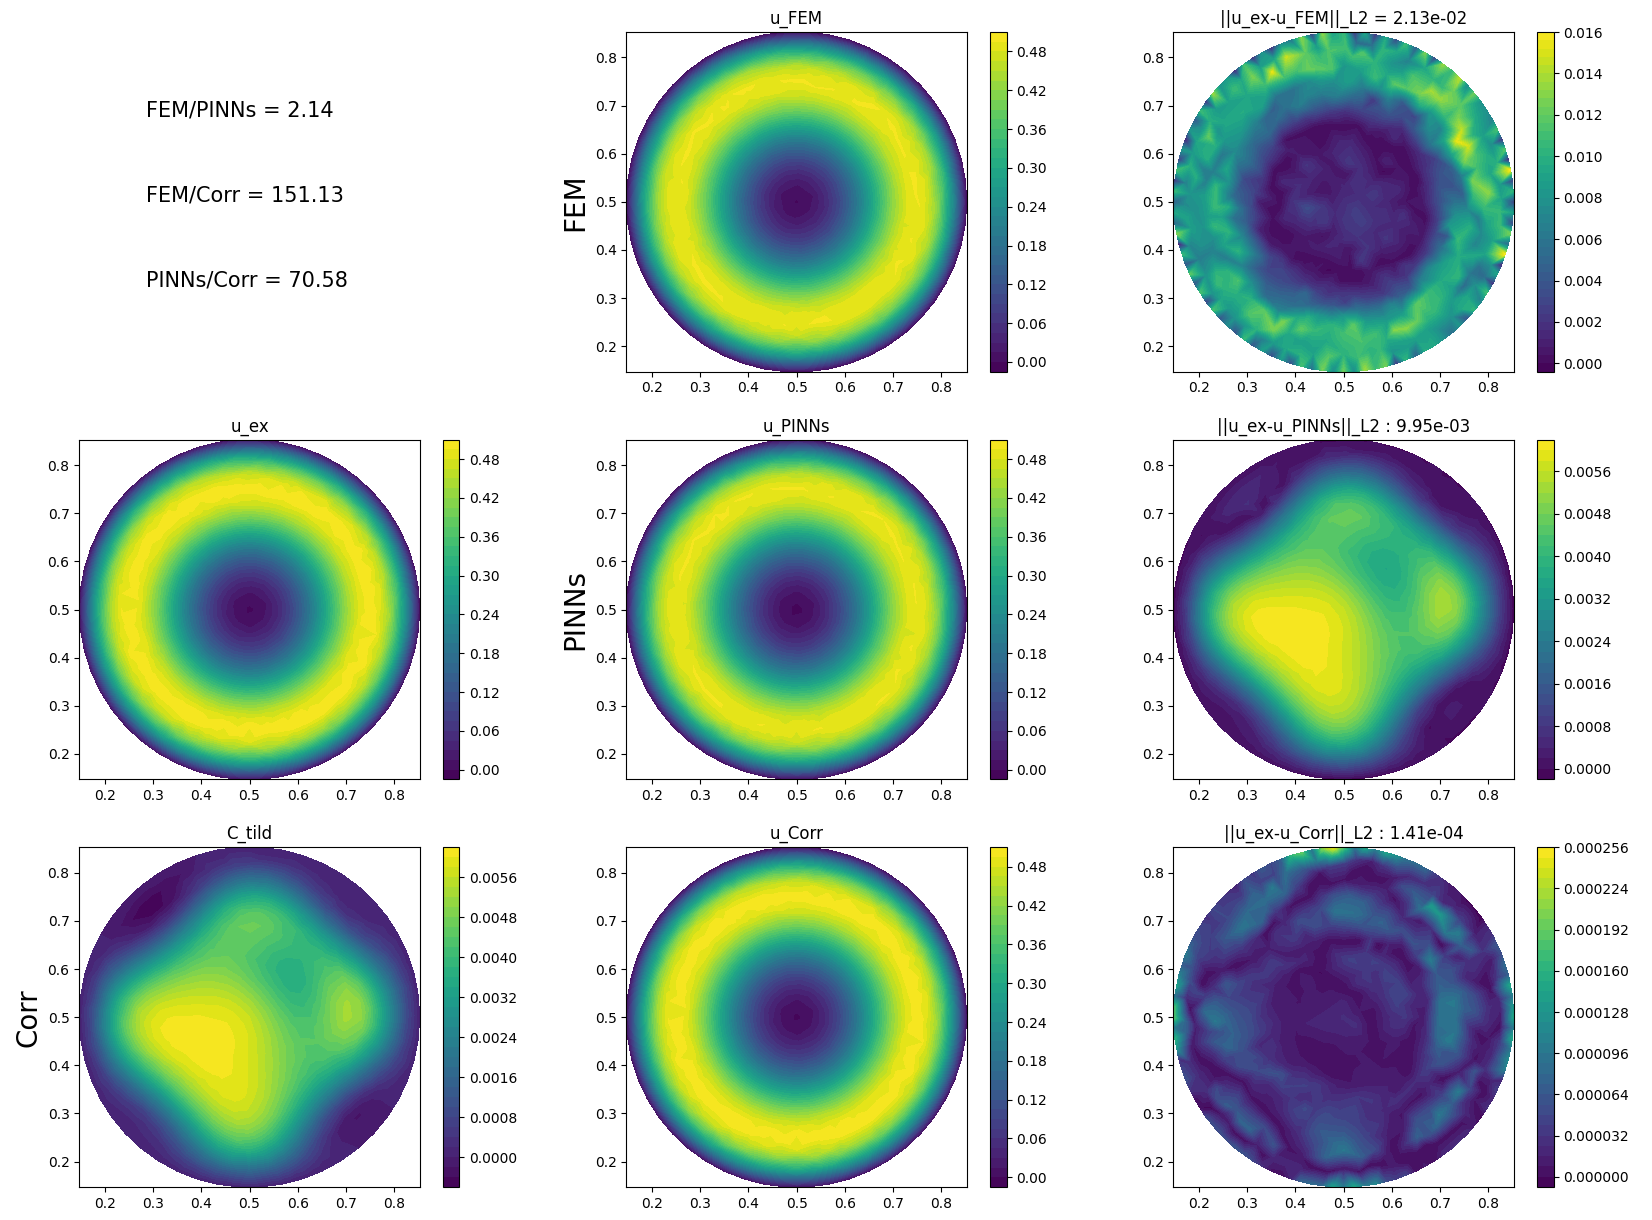
\includegraphics[width=\linewidth]{"train_sur_carre/Cercle_corr_fem_0_exact_bc.png"}
			\caption{Correction avec FEM (en apprenant sur le cercle).}
		\end{figure}
	\end{minipage}
	\begin{minipage}{0.48\linewidth}
		\begin{figure}[H]
			\centering
			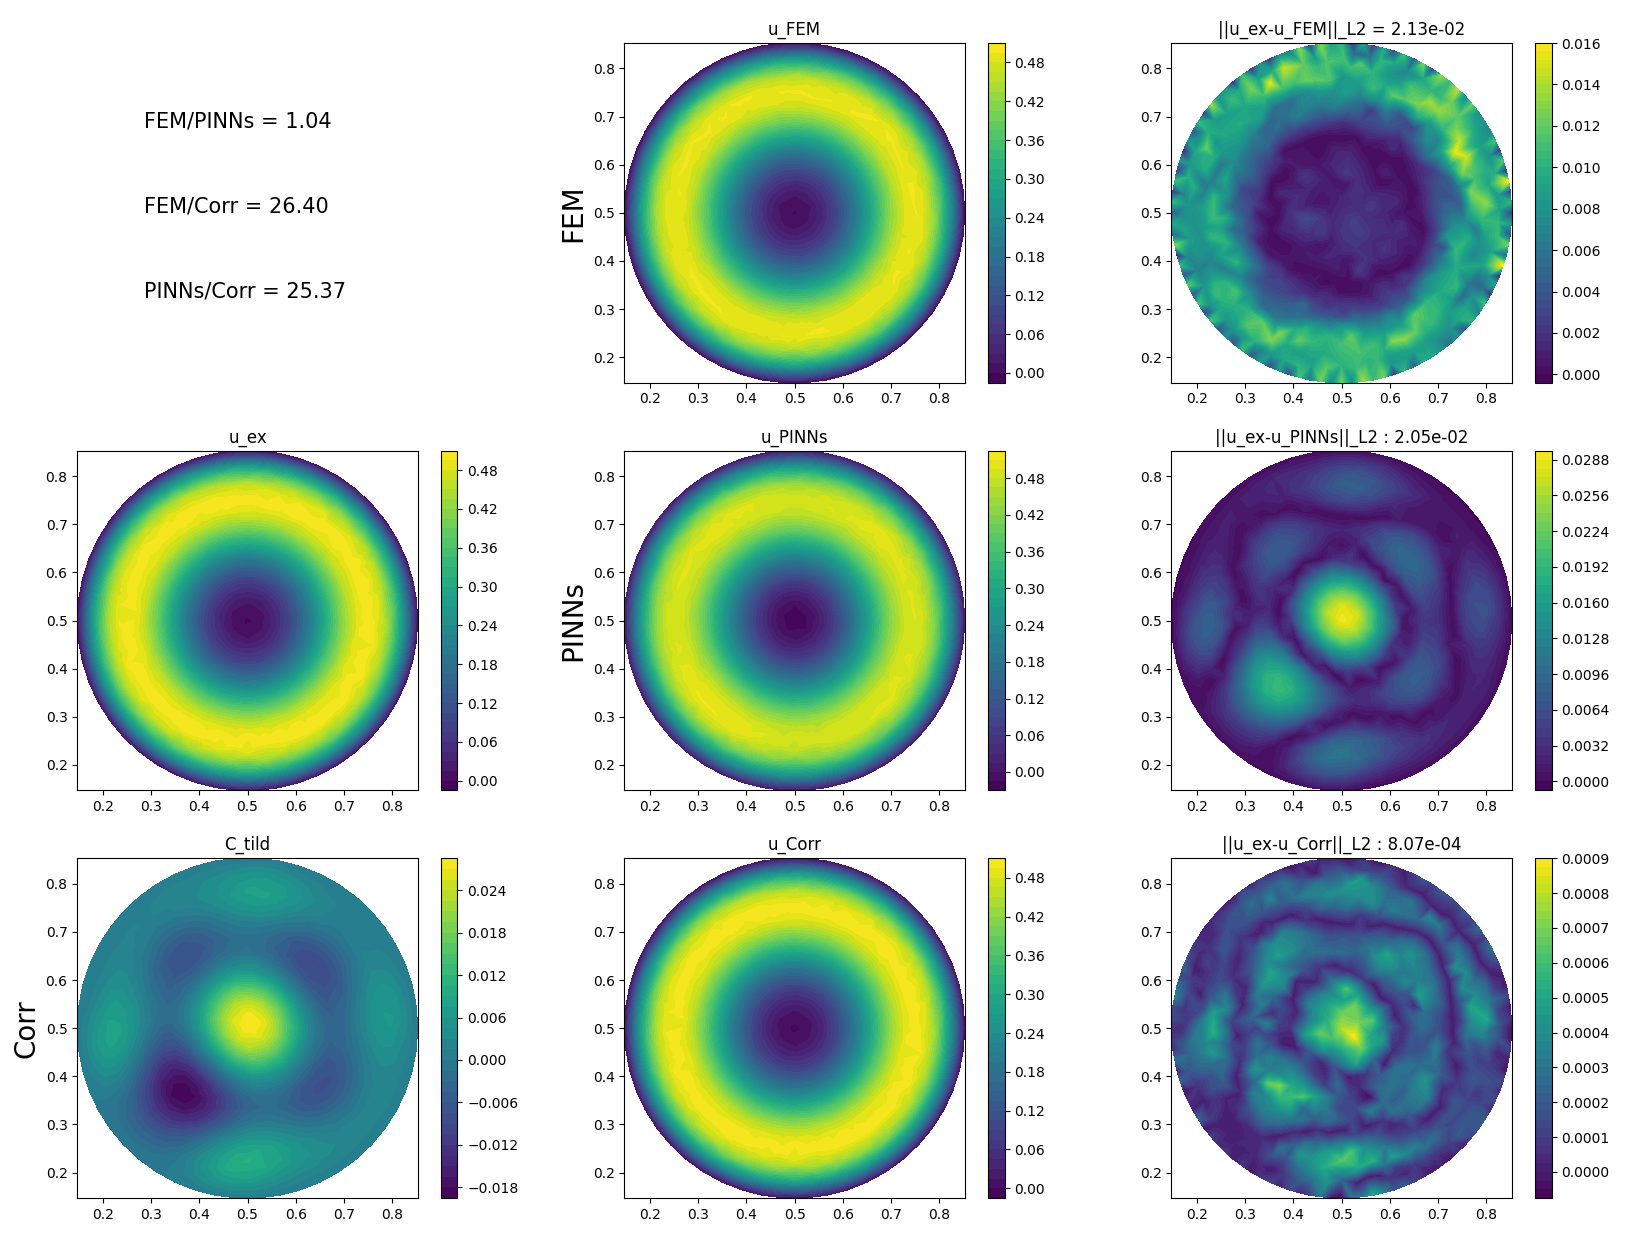
\includegraphics[width=\linewidth]{"train_sur_carre/Carre_corr_fem_1_exact_bc.png"}
			\caption{Correction avec FEM (en apprenant sur le carré).}
		\end{figure}
	\end{minipage}
\end{center}

\begin{Obs}
	Cas entraînement sur le carré (VS entraînement sur le cercle):
	\begin{itemize}
		\item PINNs $\searrow$
		\item correction avec FEM sur la prédiction $\searrow$
		\item précision finale en comparaison de FEM standard $\searrow$
	\end{itemize}
\end{Obs}

Pour $S=0.5$, on obtient les résultats suivants pour la correction par addition avec $\phi$-FEM :

\begin{minipage}{0.48\linewidth}
	\begin{figure}[H]
		\centering
		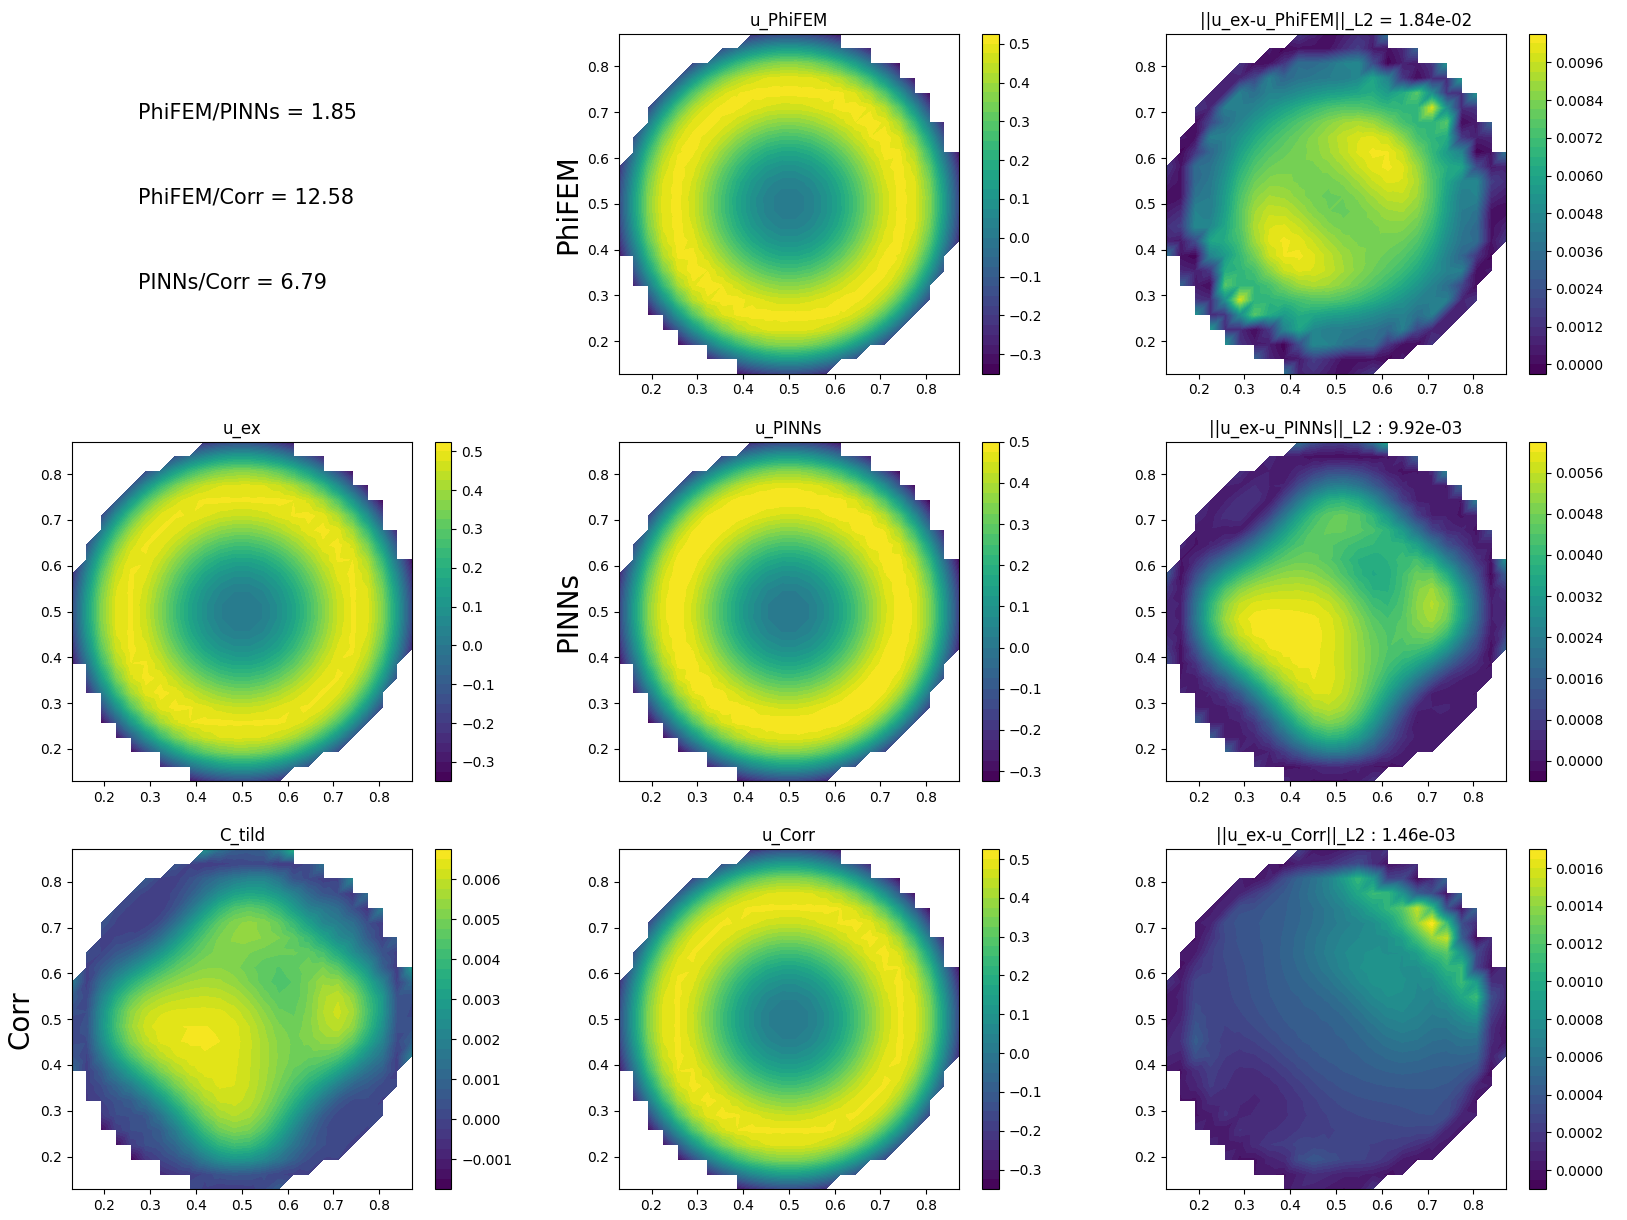
\includegraphics[width=\linewidth]{"train_sur_carre/Cercle_corr_phifem_0_exact_bc.png"}
		\caption{Correction avec $\phi$-FEM (en apprenant sur le cercle).}
	\end{figure}
\end{minipage}
\begin{minipage}{0.48\linewidth}
	\begin{figure}[H]
		\centering
		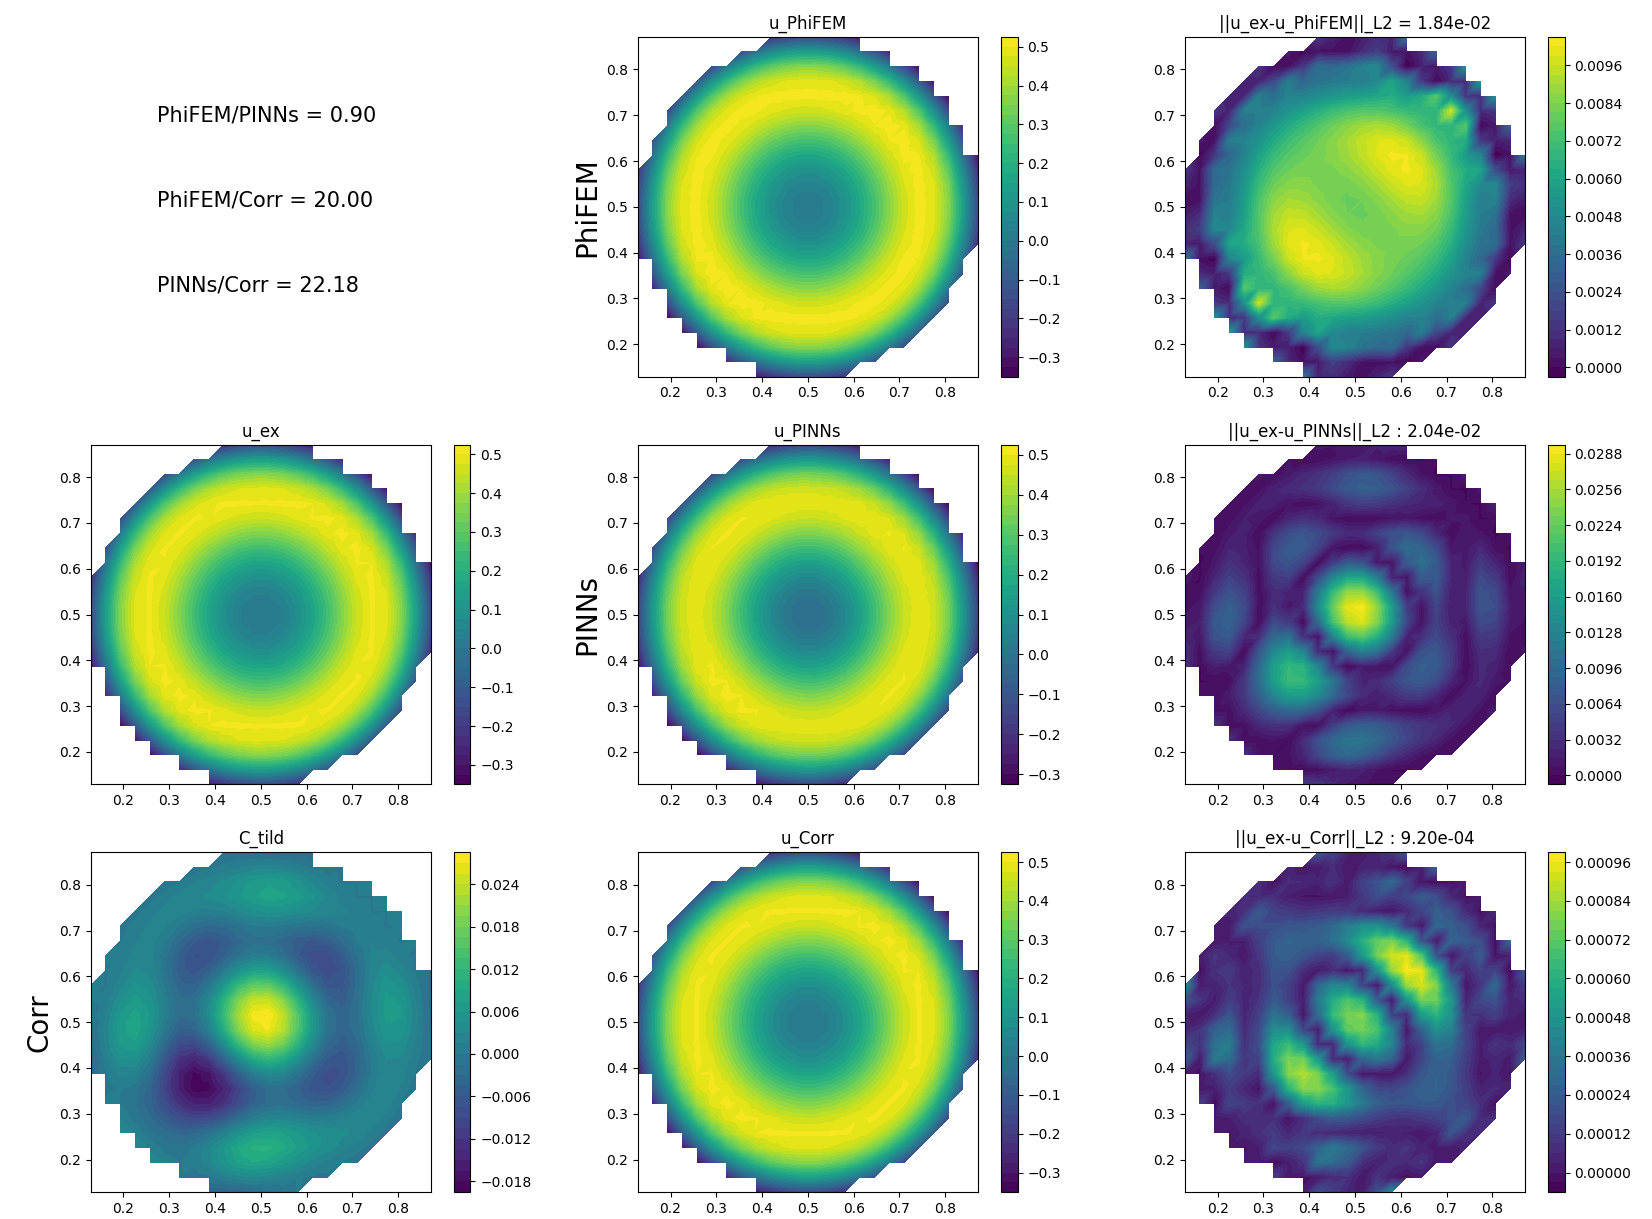
\includegraphics[width=\linewidth]{"train_sur_carre/Carre_corr_phifem_1_exact_bc.png"}
		\caption{Correction avec $\phi$-FEM (en apprenant sur le carré).}
	\end{figure}
\end{minipage}

\begin{Obs}
	Cas entraînement sur le carré (VS entraînement sur le cercle):
	\begin{itemize}
		\item PINNs $\searrow$ (moins bon que $\phi$-FEM standard)
		\item correction avec $\phi$-FEM sur la prédiction $\nearrow$
		\item précision finale en comparaison de $\phi$-FEM standard $\nearrow$
	\end{itemize}
	+ précision finale pour FEM et $\phi$-FEM du même ordre
\end{Obs}

Pour $\phi$-FEM on s'intéresse en fait à l'erreur sur $\Omega$ (et non $\Omega_h$), voici les résultats obtenus en projetant la solution sur $\Omega$ :

\begin{figure}[H]
	\centering
	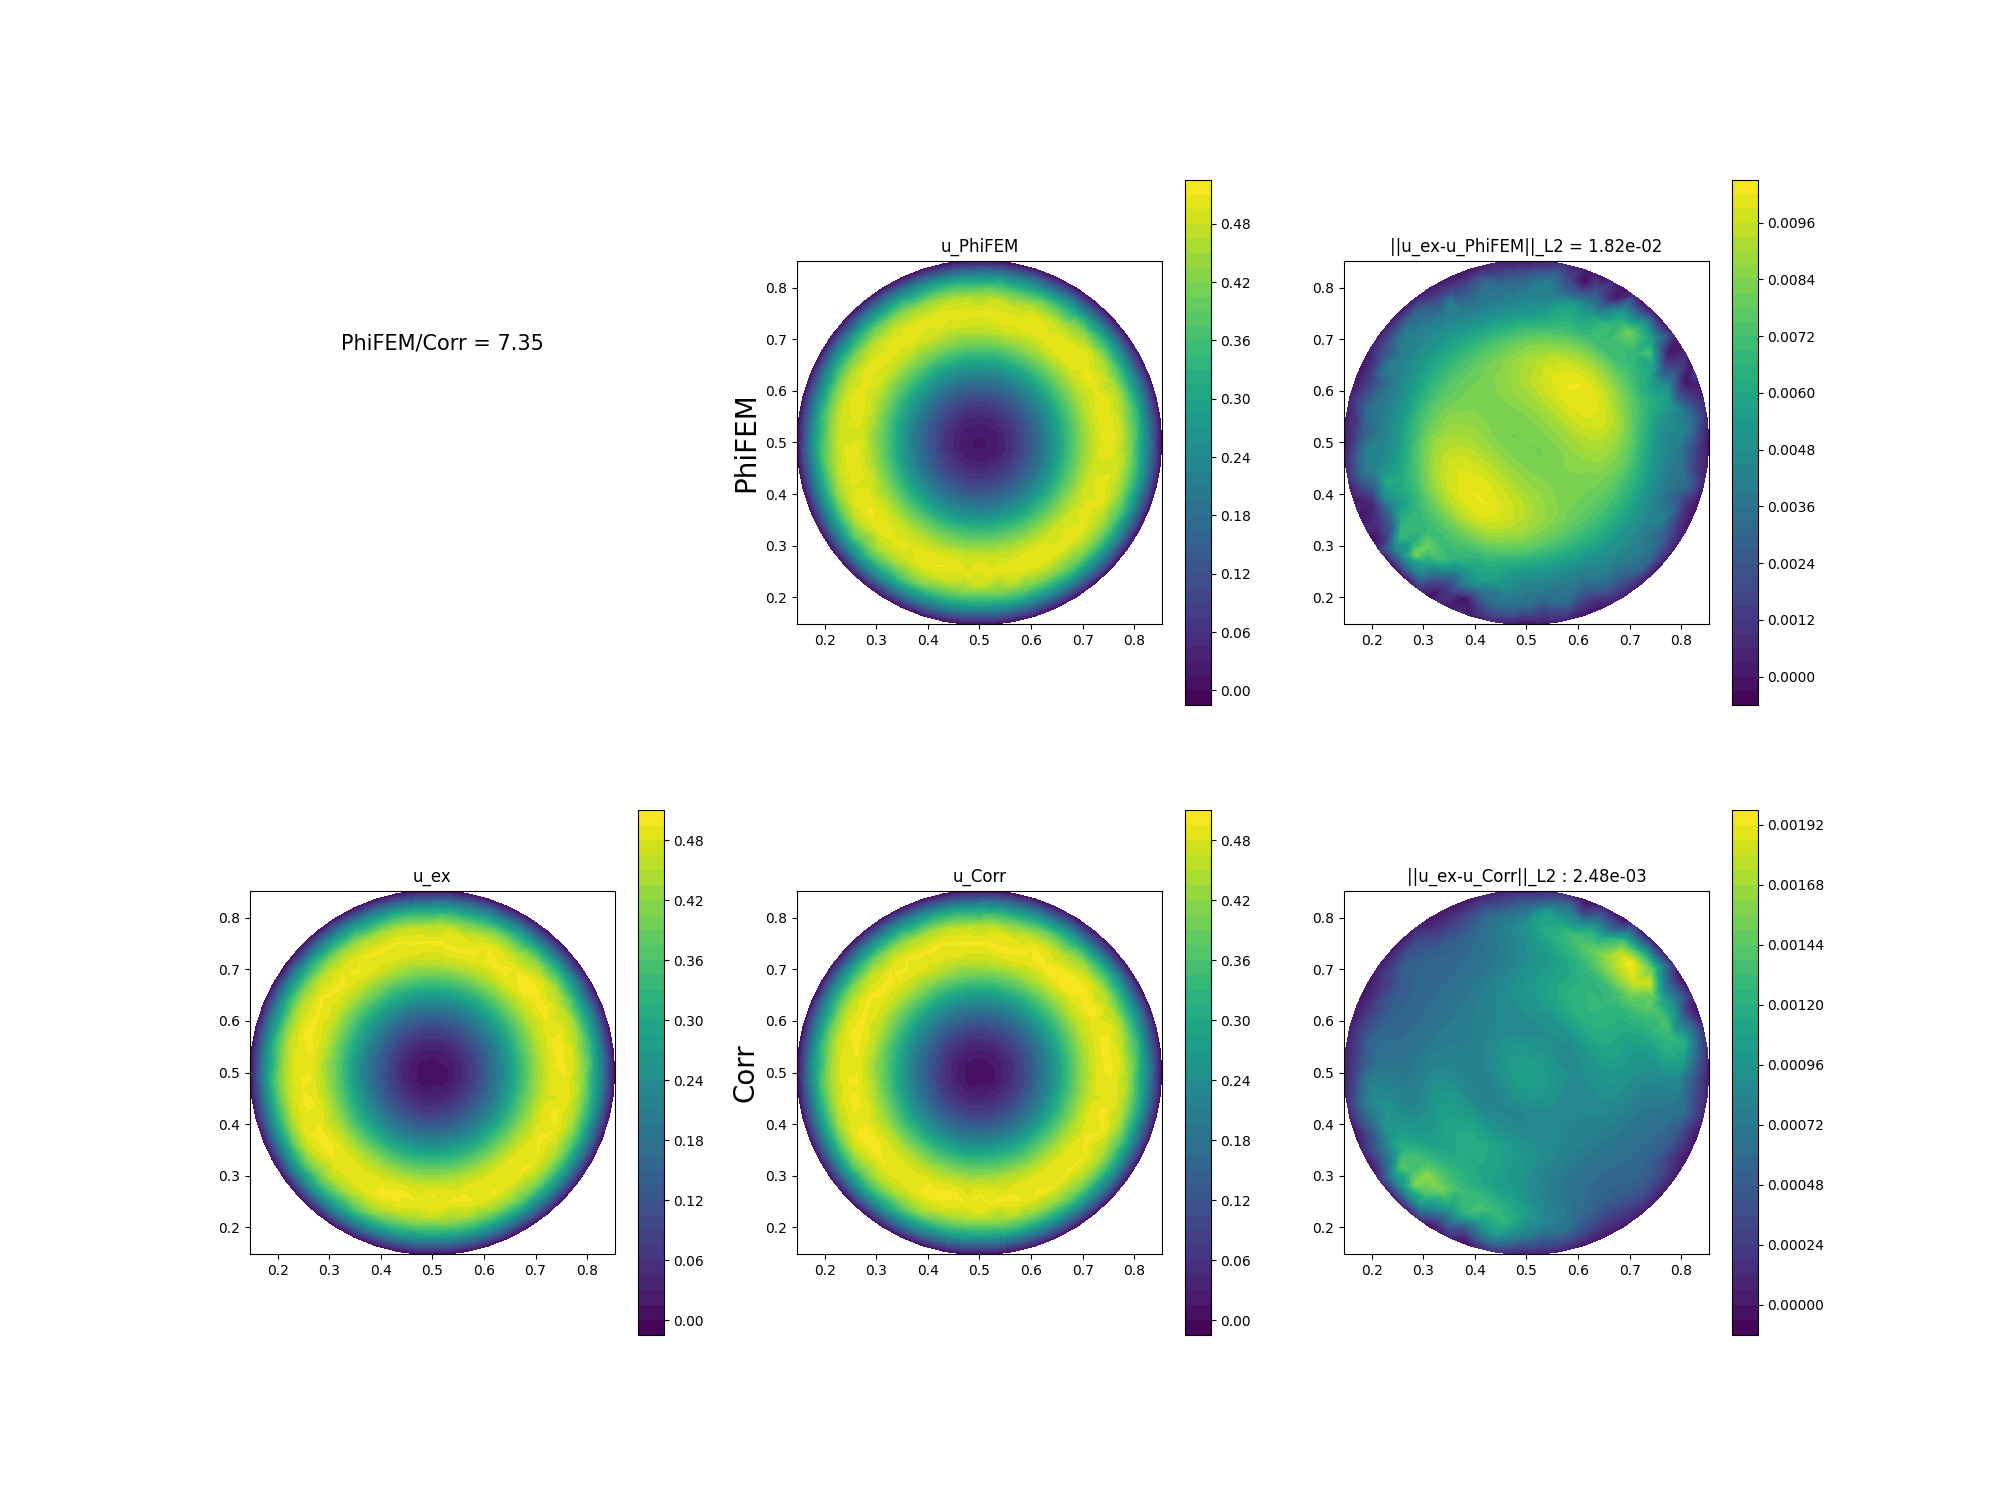
\includegraphics[width=0.5\linewidth]{"train_sur_carre/corr_phifem_1_Omega_exact_bc.png"}
	\caption{Correction avec $\phi$-FEM (en apprenant sur le carré) - projection sur $\Omega$.}
\end{figure}

\begin{Obs}
	Résultats assez similaire sur $\Omega$ et $\Omega_h$.
\end{Obs}

\newpage

\subsection{Correction sur la prédiction du modèle sur $u$ avec recalage de la fonction levelset}

\begin{minipage}{0.58\linewidth}
	On sélectionne des points assez proche du bord puis on fait une descente de gradient (en quelque sorte à pas optimale) sur 50 itérations dans le but de recaler la levelset sur le bord :
	\begin{equation*}
		\begin{pmatrix}
			x \\
			y
		\end{pmatrix}\leftarrow\begin{pmatrix}
			x \\
			y
		\end{pmatrix}-\phi(x,y)\cdot\nabla\phi(x,y)
	\end{equation*}
\end{minipage}
\begin{minipage}{0.38\linewidth}
	\begin{figure}[H]
		\centering
		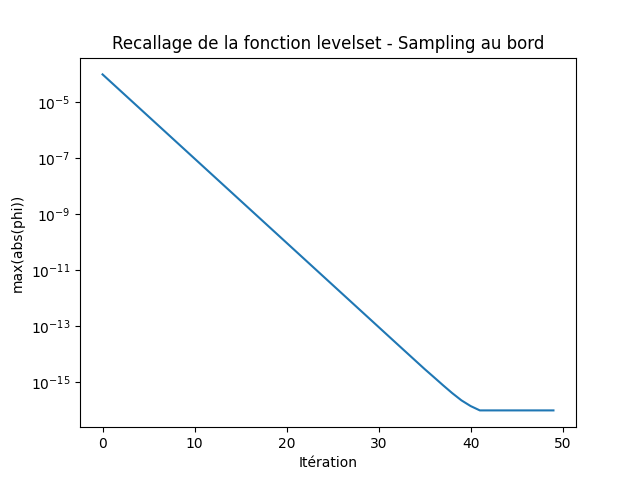
\includegraphics[width=0.8\linewidth]{"recalage_levelset/erreur_iterations.png"}
		\caption{Valeur maximale de la levelset en fonction des itérations.}
	\end{figure}
\end{minipage}



\begin{Obs}
	A la fin, la valeur maximale de $\phi$ en les points choisis (en valeur absolu) est de 1e-17.
\end{Obs}

En entraînant le modèle avec les paramètres par défaut (CONFIG 0) à apprendre $u$ uniquement sur $\Omega$ (avec loss = loss résidu + loss bc), on obtient les résultats d'entraînement suivant - à gauche : sans recalage / à droite avec recalage :

\begin{minipage}{0.48\linewidth}
	\begin{figure}[H]
		\centering
		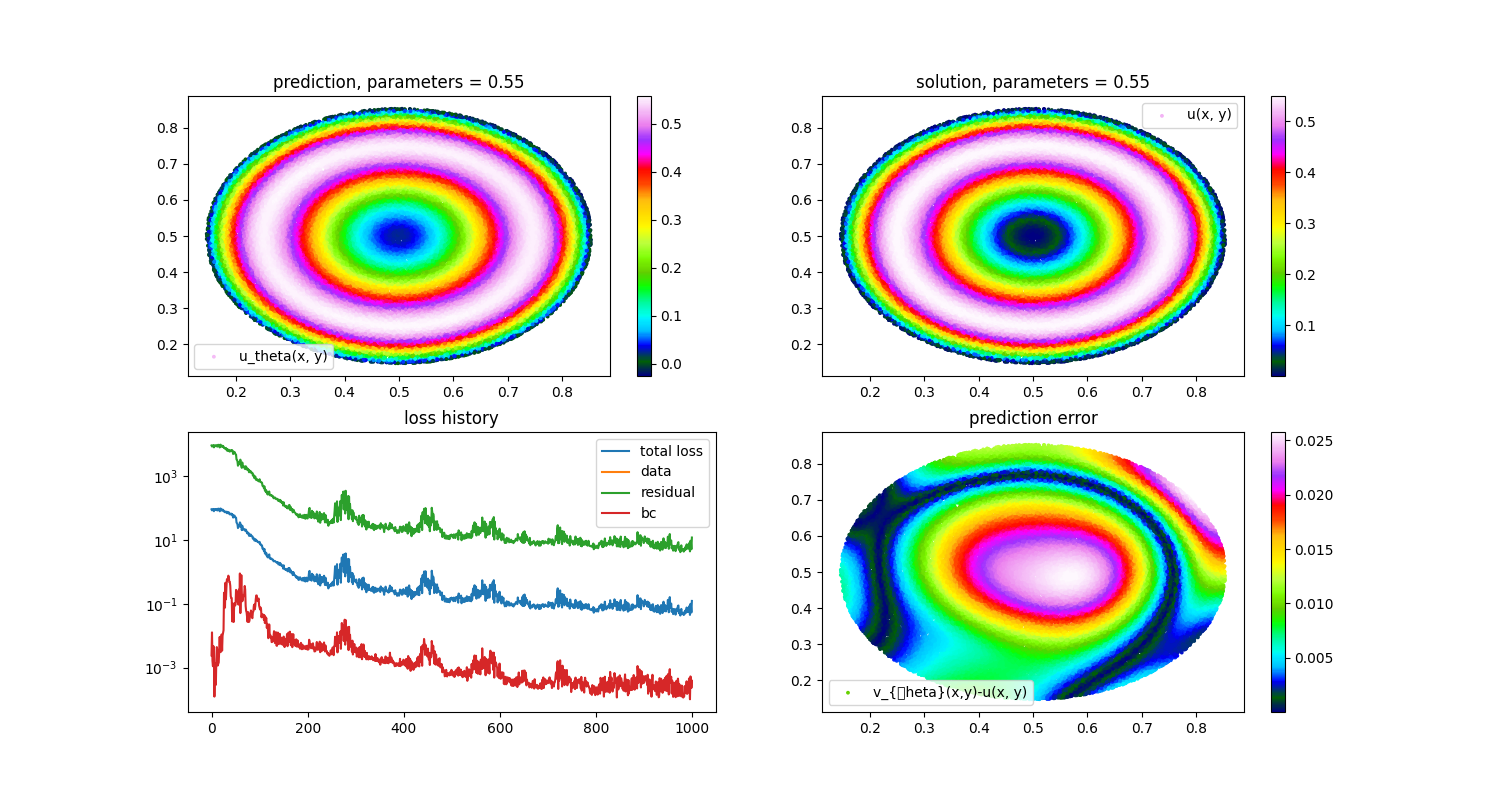
\includegraphics[width=\linewidth]{"recalage_levelset/model_0.png"}
		\caption{Entraînement sans recalage de la levelset.}
	\end{figure}
\end{minipage}
\begin{minipage}{0.48\linewidth}
	\begin{figure}[H]
		\centering
		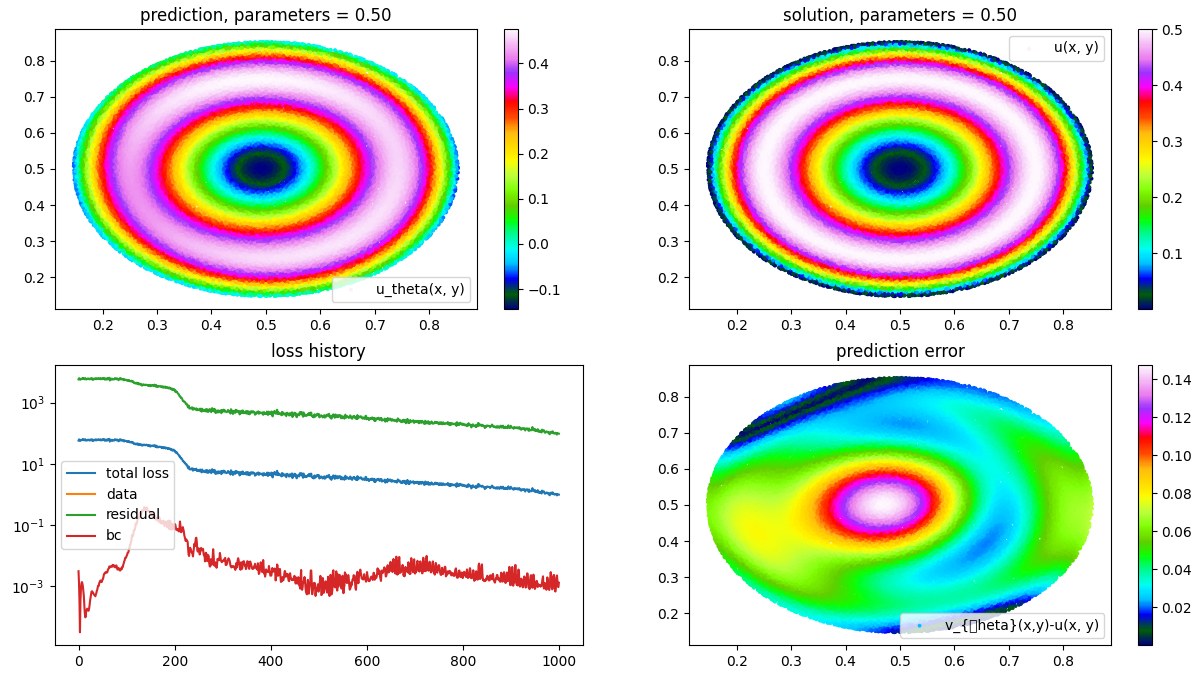
\includegraphics[width=\linewidth]{"recalage_levelset/model_0_align_levelset.png"}
		\caption{Entraînement avec recalage de la levelset.}
	\end{figure}
\end{minipage}

\begin{Obs}
	Il semblerait que l'entrainement du modèle avec recalage de la levelset ne fournisse pas les résultats attendus.
\end{Obs}

On essaye de ré-entraîner le modèle en modifiant les paramètres de la manière suivante (CONFIG 2) :

\begin{figure}[H]
	\centering
	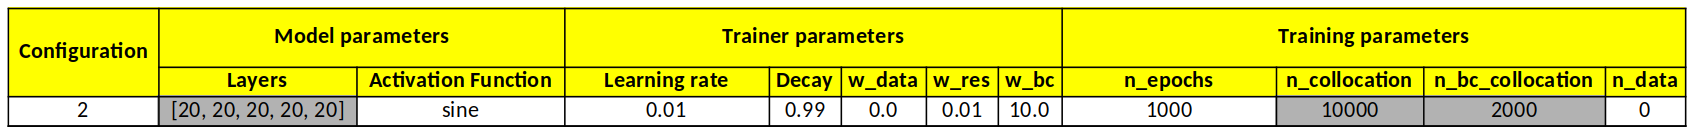
\includegraphics[width=0.8\linewidth]{"recalage_levelset/config_align_levelset.png"}
	\caption{Paramètres du PINNs.}
\end{figure}

On obtient les résultats d'entraînement suivant :

\begin{figure}[H]
	\centering
	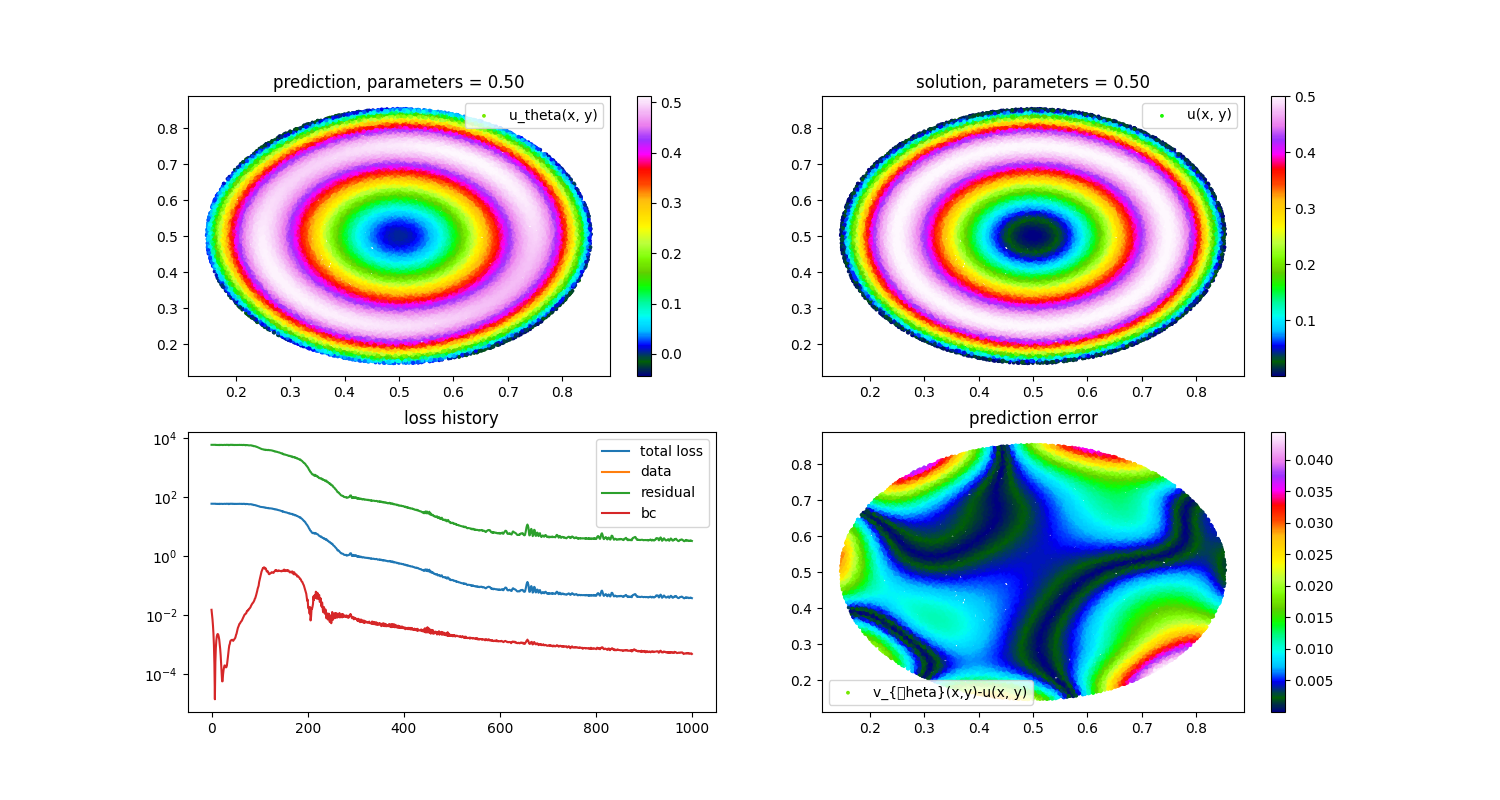
\includegraphics[width=0.45\linewidth]{"recalage_levelset/model_2_align_levelset.png"}
	\caption{Entraînement avec recalage de la levelset.}
\end{figure}

Pour $S=0.5$, on obtient les résultats suivants pour la correction par addition avec FEM - à gauche : sans recalage (CONFIG 0) / à droite : avec recalage (CONFIG 2) :

\begin{minipage}{0.48\linewidth}
	\begin{figure}[H]
		\centering
		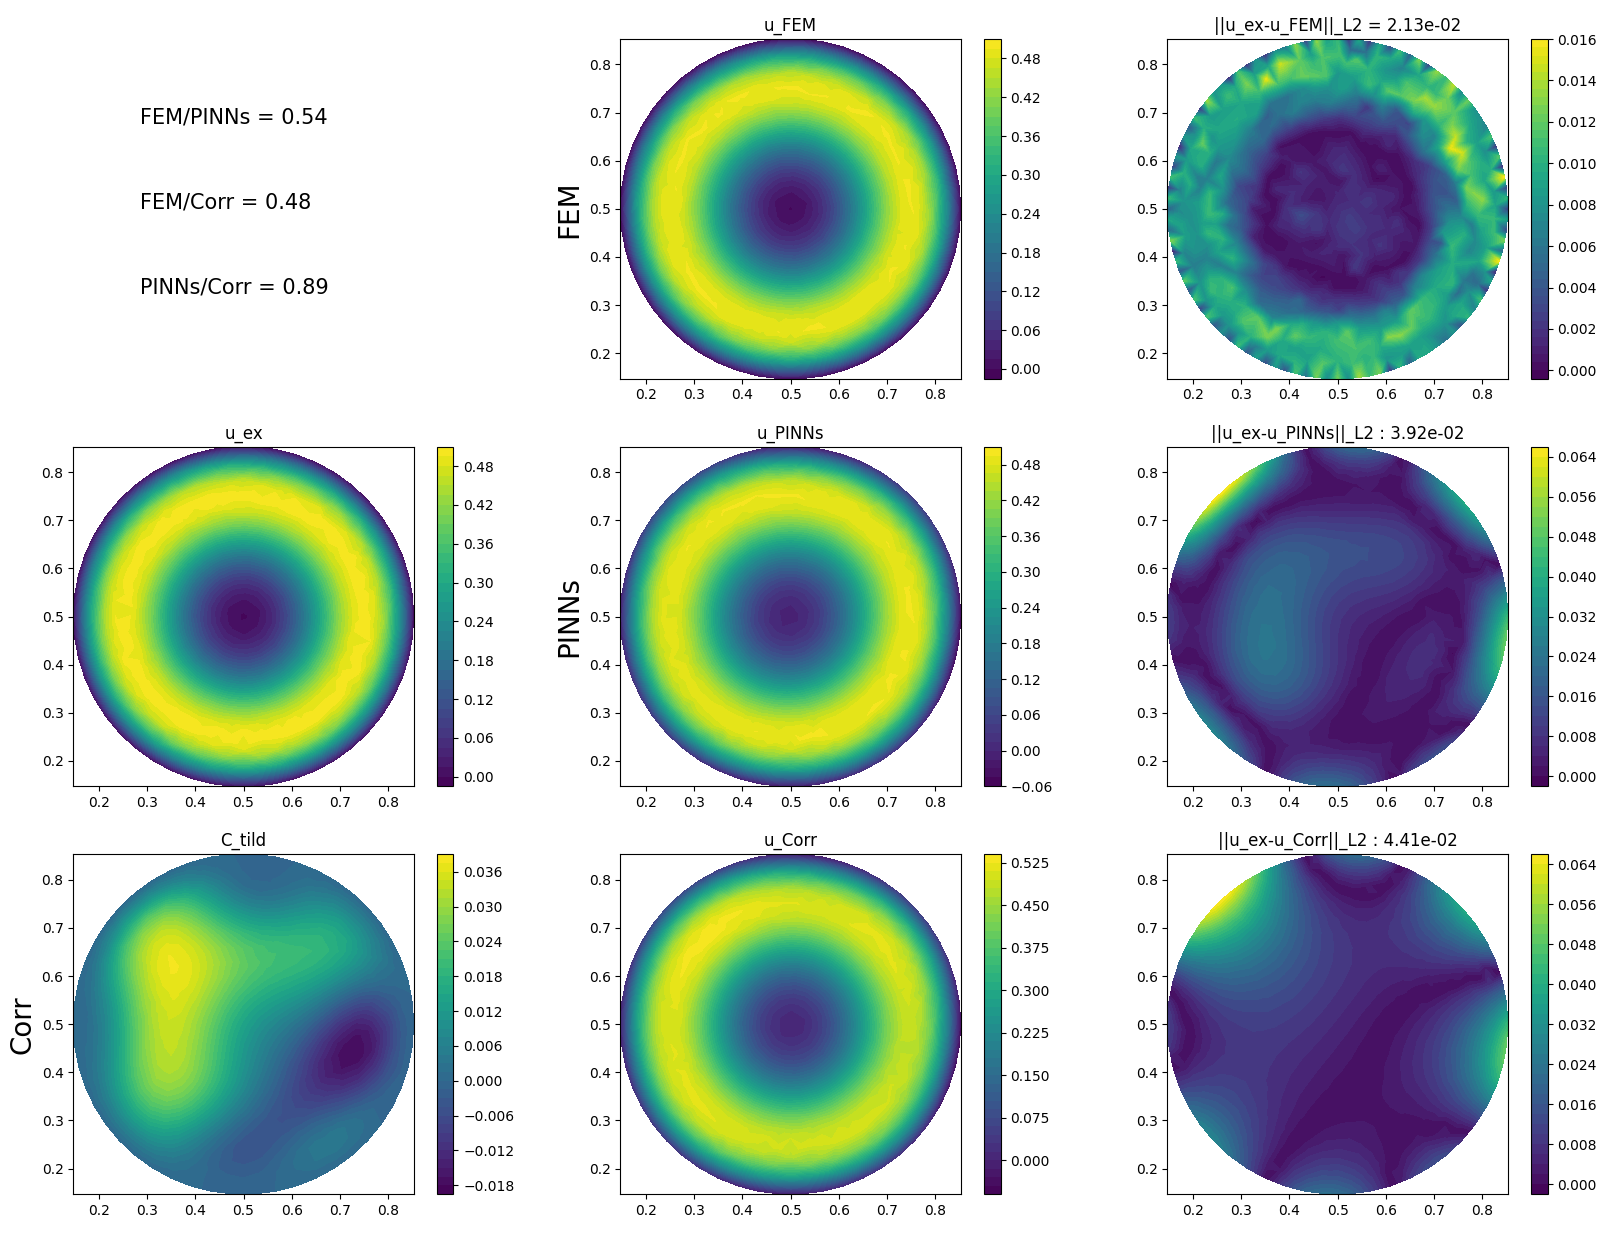
\includegraphics[width=\linewidth]{"recalage_levelset/corr_fem_0.png"}
		\caption{Correction avec FEM (sans recalage - CONFIG 0).}
	\end{figure}
\end{minipage}
\begin{minipage}{0.48\linewidth}
	\begin{figure}[H]
		\centering
		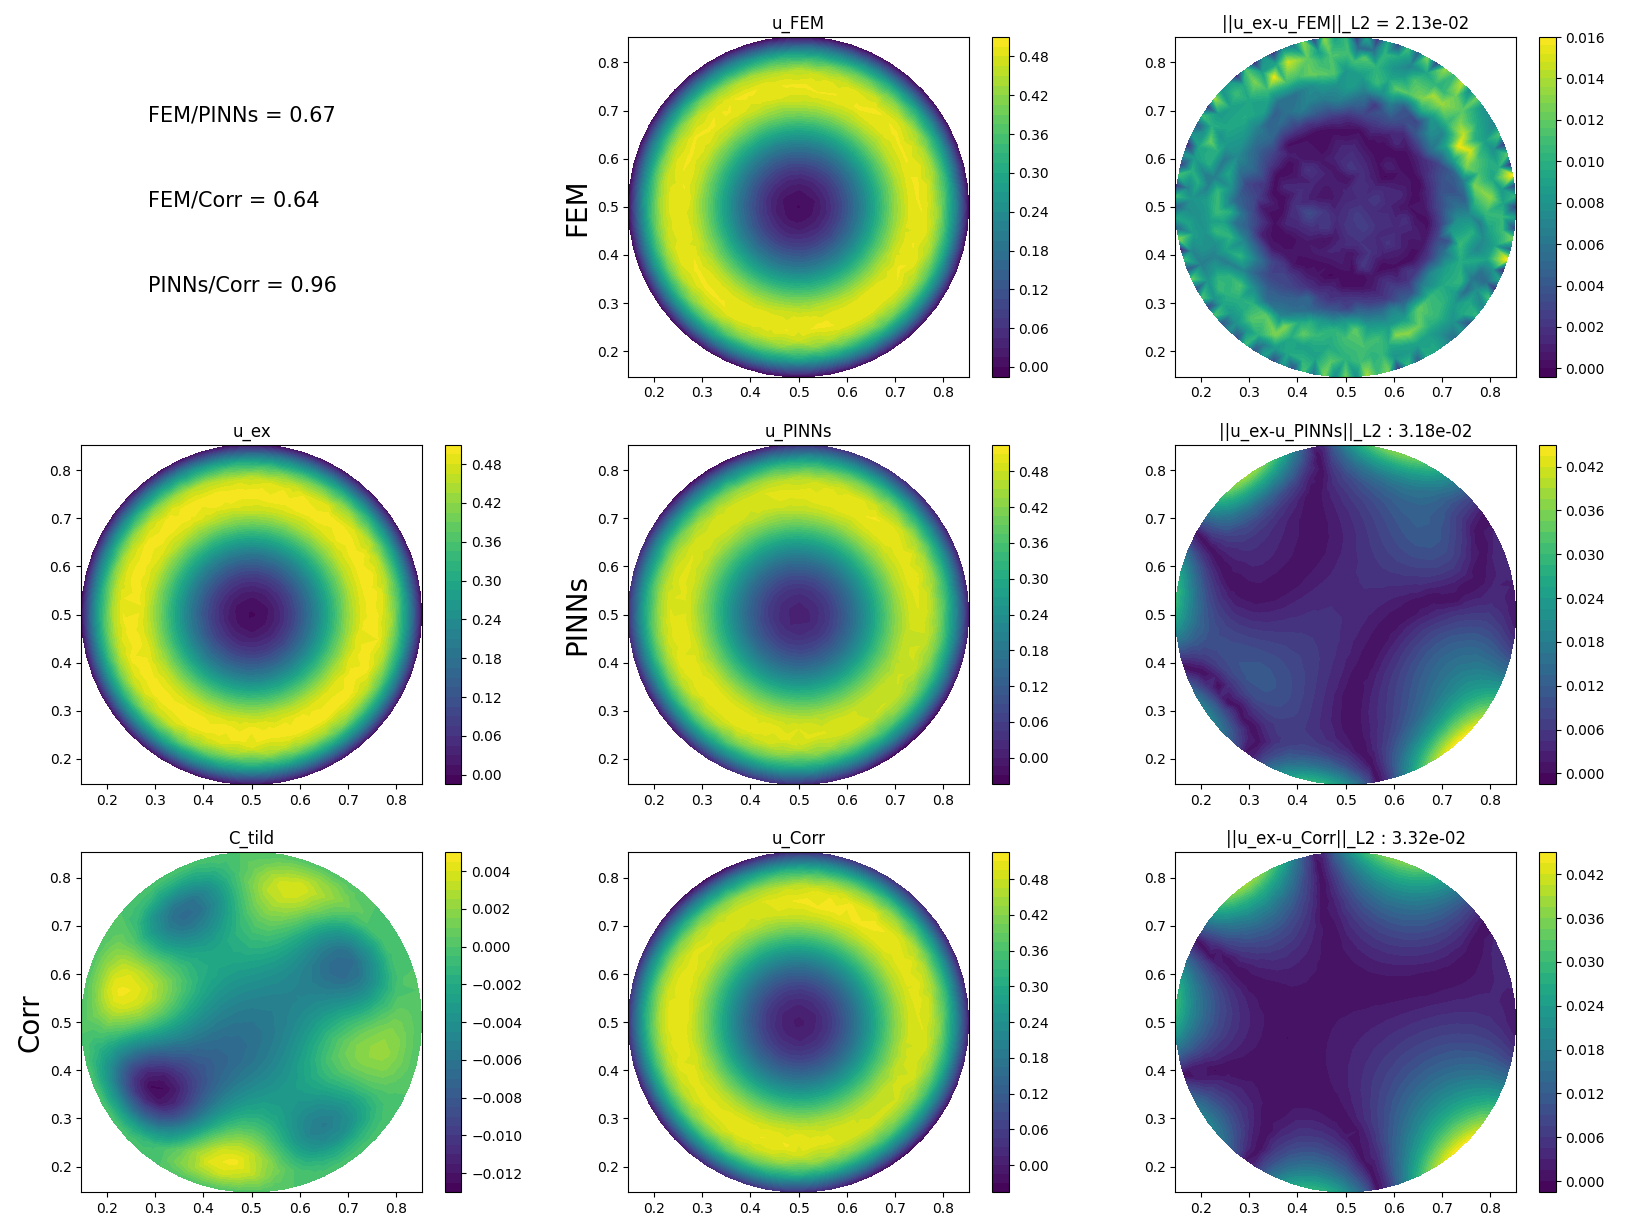
\includegraphics[width=\linewidth]{"recalage_levelset/corr_fem_2_align_levelset.png"}
		\caption{Correction avec FEM (avec recalage - CONFIG 2).}
	\end{figure}
\end{minipage}

\begin{Obs}
	Cas avec recalage (VS sans recalage):
	\begin{itemize}
		\item PINNs $\nearrow$ (moins bon que FEM standard)
		\item correction avec FEM sur la prédiction $\nearrow$
		\item précision finale en comparaison de FEM standard $\nearrow$
	\end{itemize}
	
	On remarque tout de même que les résultats sont très insuffisant mais très similaire.
	
	ATTENTION : On ne compare pas les mêmes modèles ici (pas les mêmes configs).
\end{Obs}

\subsection{Variation du terme source $f$}

On veut faire varier le second membre en prenant $S\in[0.1,1]$. On considère la configuration par défaut et on apprend $u=\phi w$.

Pour $S=0.55$ (car moyenne des paramètres), on obtient les résultats d'entraînement suivant - à gauche : avec $f$ fixé / à droite : avec $f$ qui varie :

\begin{minipage}{0.48\linewidth}
	\begin{figure}[H]
		\centering
		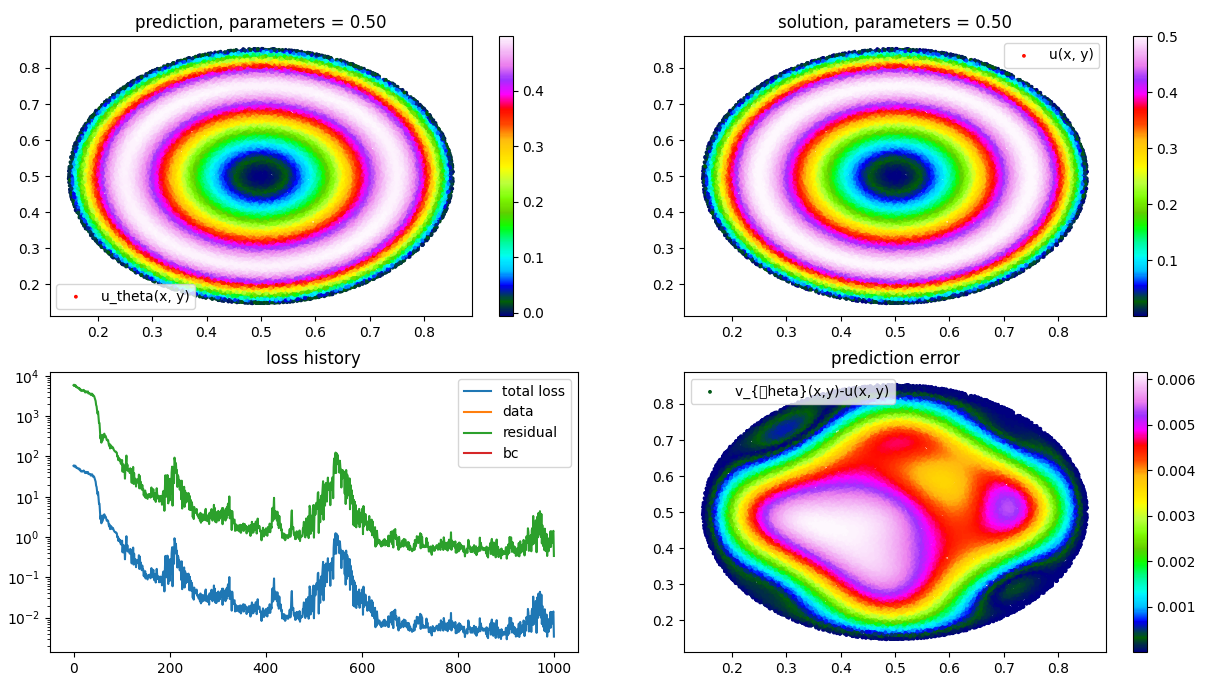
\includegraphics[width=\linewidth]{"varier_f/Poisson2D_fixed_model_0_exact_bc.png"}
		\caption{Training $f$ fixé.}
	\end{figure}
\end{minipage}
\begin{minipage}{0.48\linewidth}
	\begin{figure}[H]
		\centering
		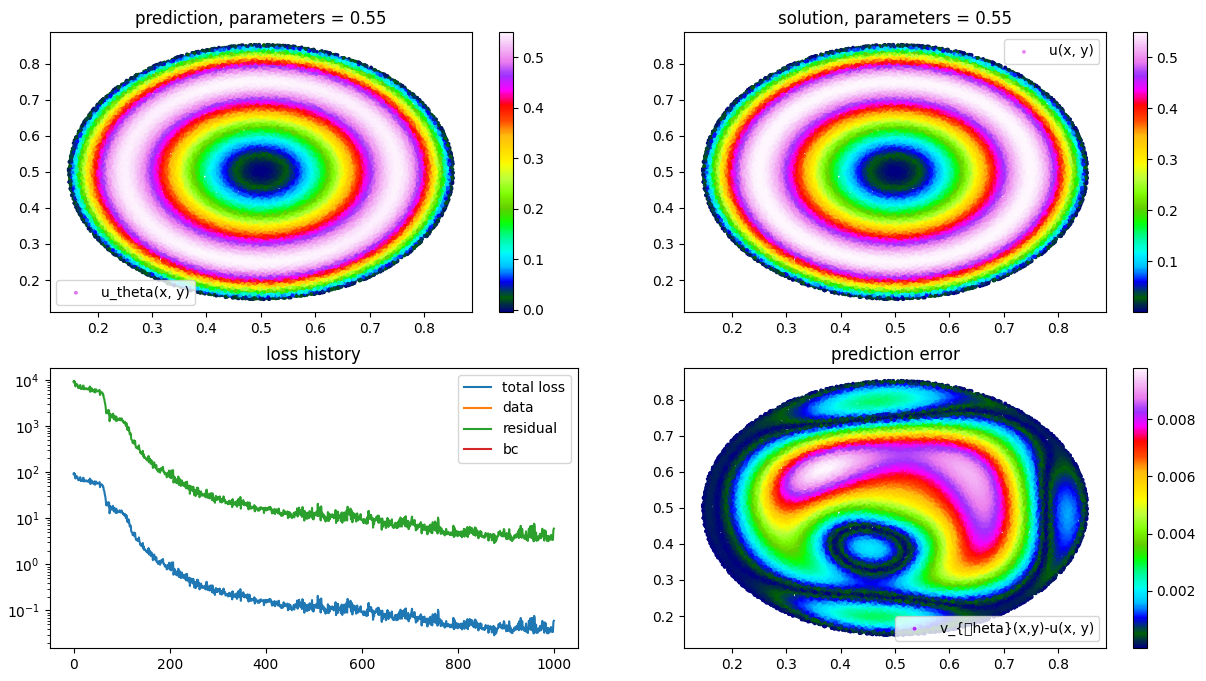
\includegraphics[width=\linewidth]{"varier_f/Poisson2D_f_model_0_exact_bc.png"}
		\caption{Training $f$ qui varie.}
	\end{figure}
\end{minipage}

\newpage

Pour $S=0.5$, on obtient les résultats suivants pour la correction par addition avec FEM :

\begin{minipage}{0.48\linewidth}
	\begin{figure}[H]
		\centering
		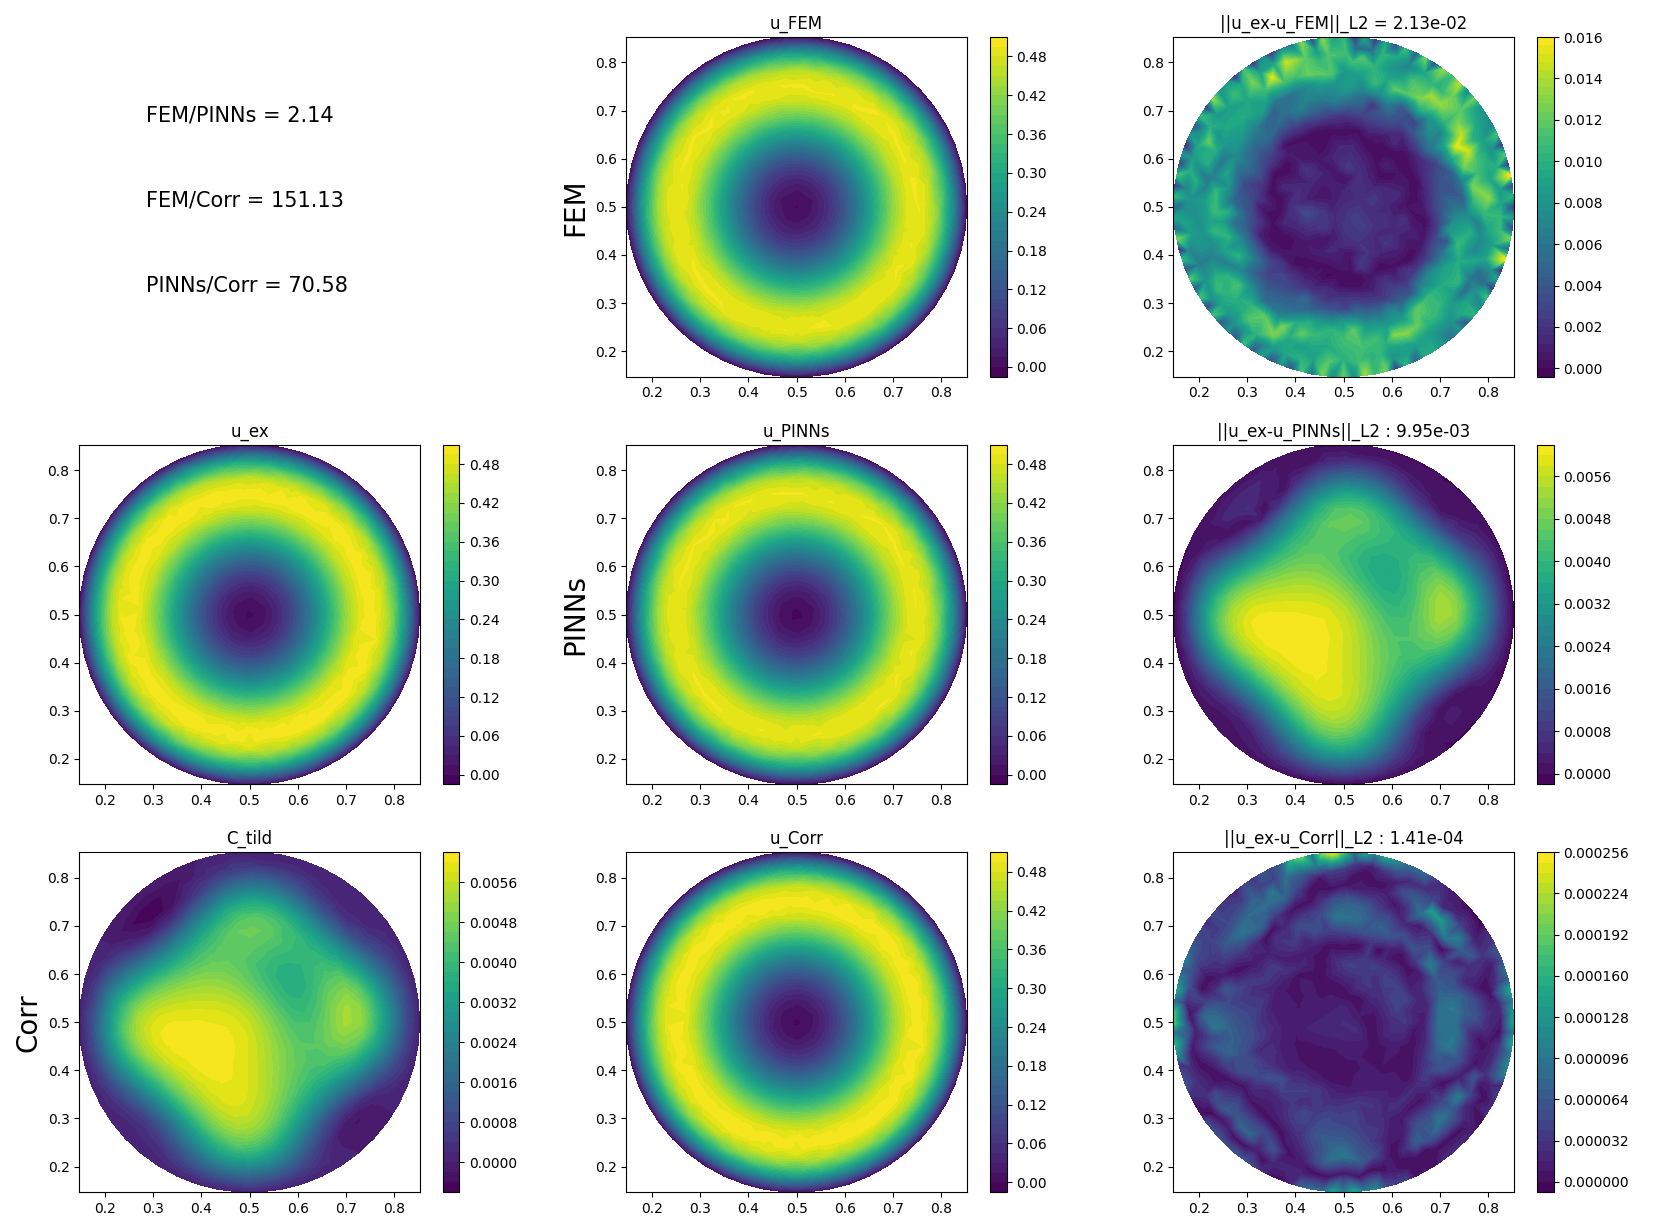
\includegraphics[width=\linewidth]{"varier_f/Poisson2D_fixed_corr_fem_0_exact_bc.png"}
		\caption{Correction avec FEM - $f$ fixé.}
		\label{Poisson2D_fixed_corr_fem_0_exact_bc}
	\end{figure}
\end{minipage}
\begin{minipage}{0.48\linewidth}
	\begin{figure}[H]
		\centering
		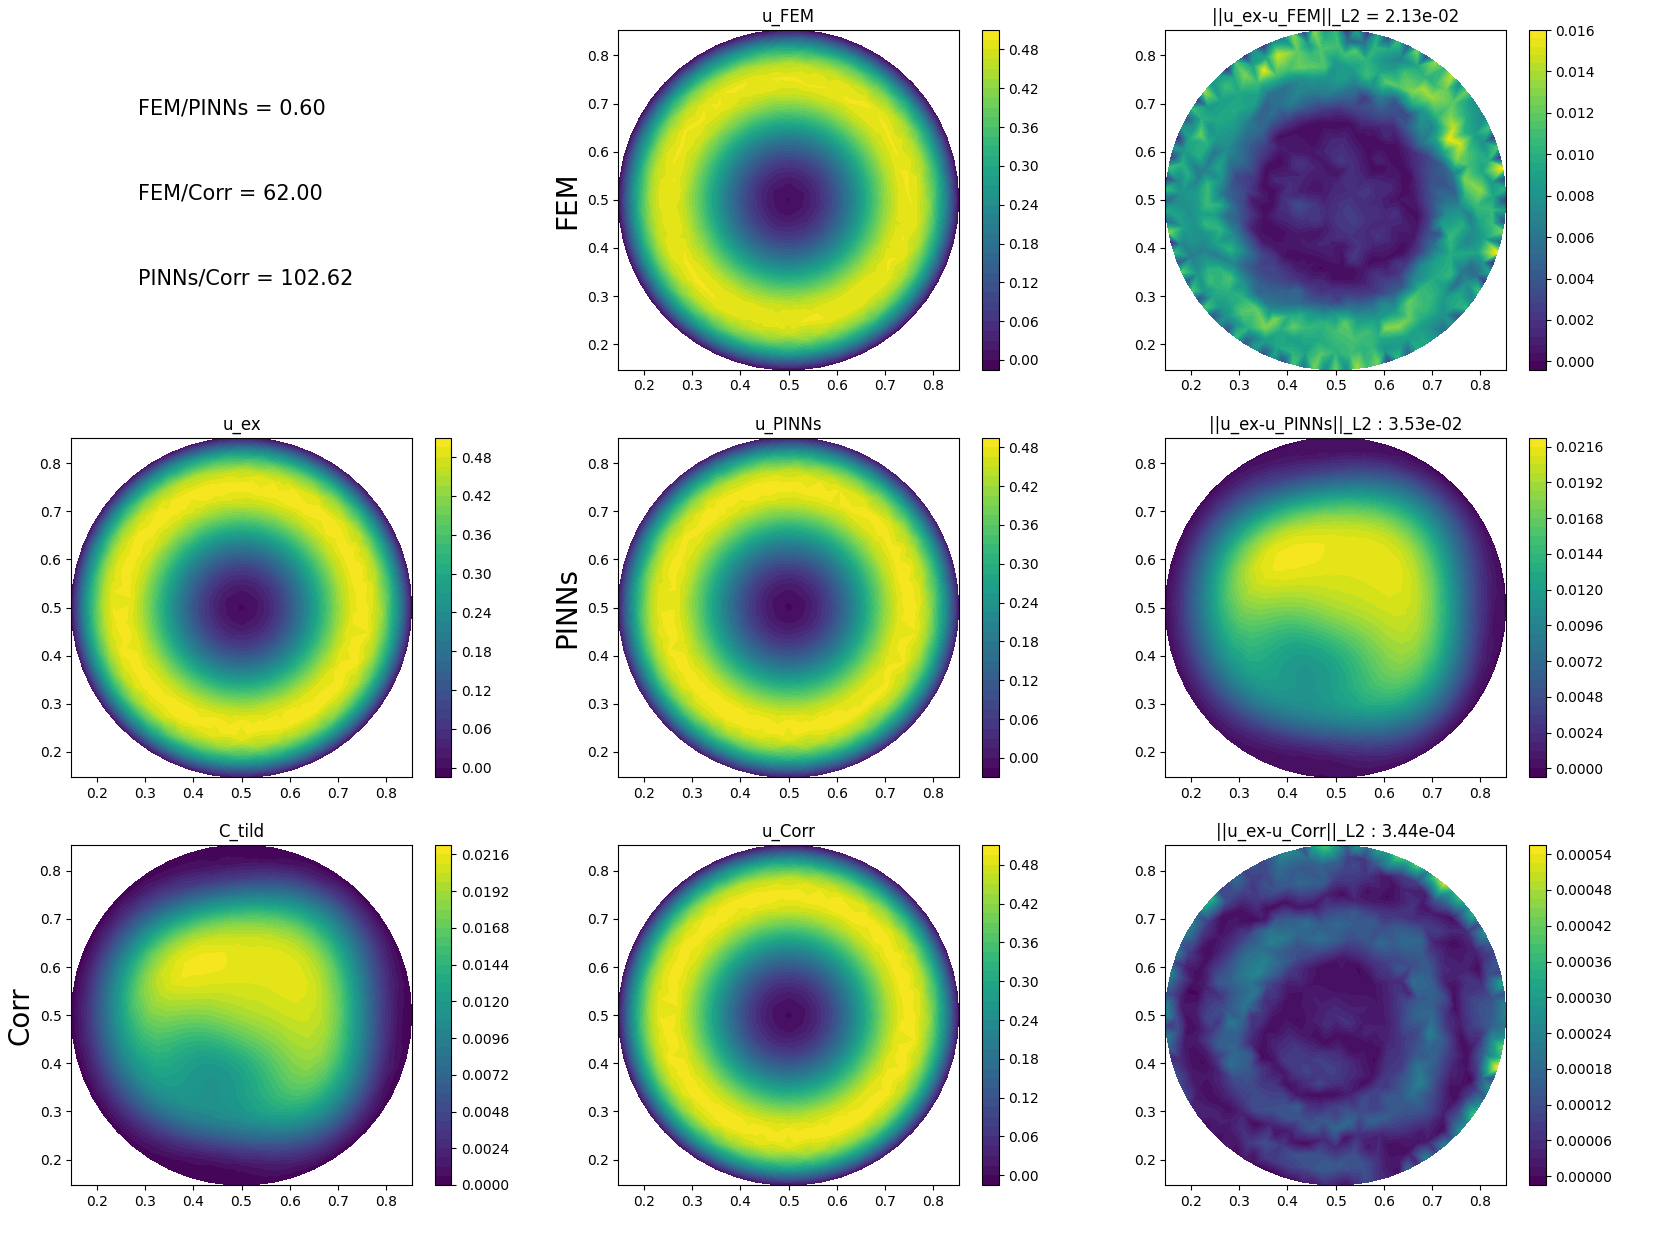
\includegraphics[width=\linewidth]{"varier_f/Poisson2D_f_corr_fem_0_exact_bc.png"}
		\caption{Correction avec FEM - $f$ qui varie.}
	\end{figure}
\end{minipage}

\begin{Obs}
	Cas $f$ qui varie (VS cas $f$ fixé) :
	\begin{itemize}
		\item PINNs $\searrow$ (moins bon que FEM standard)
		\item correction avec FEM sur la prédiction $\nearrow$ 
		\item précision finale en comparaison de FEM standard $\searrow$ 
	\end{itemize}
\end{Obs}

Pour $S=0.5$, on obtient les résultats suivants pour la correction par addition avec $\phi$-FEM :

\begin{minipage}{0.48\linewidth}
	\begin{figure}[H]
		\centering
		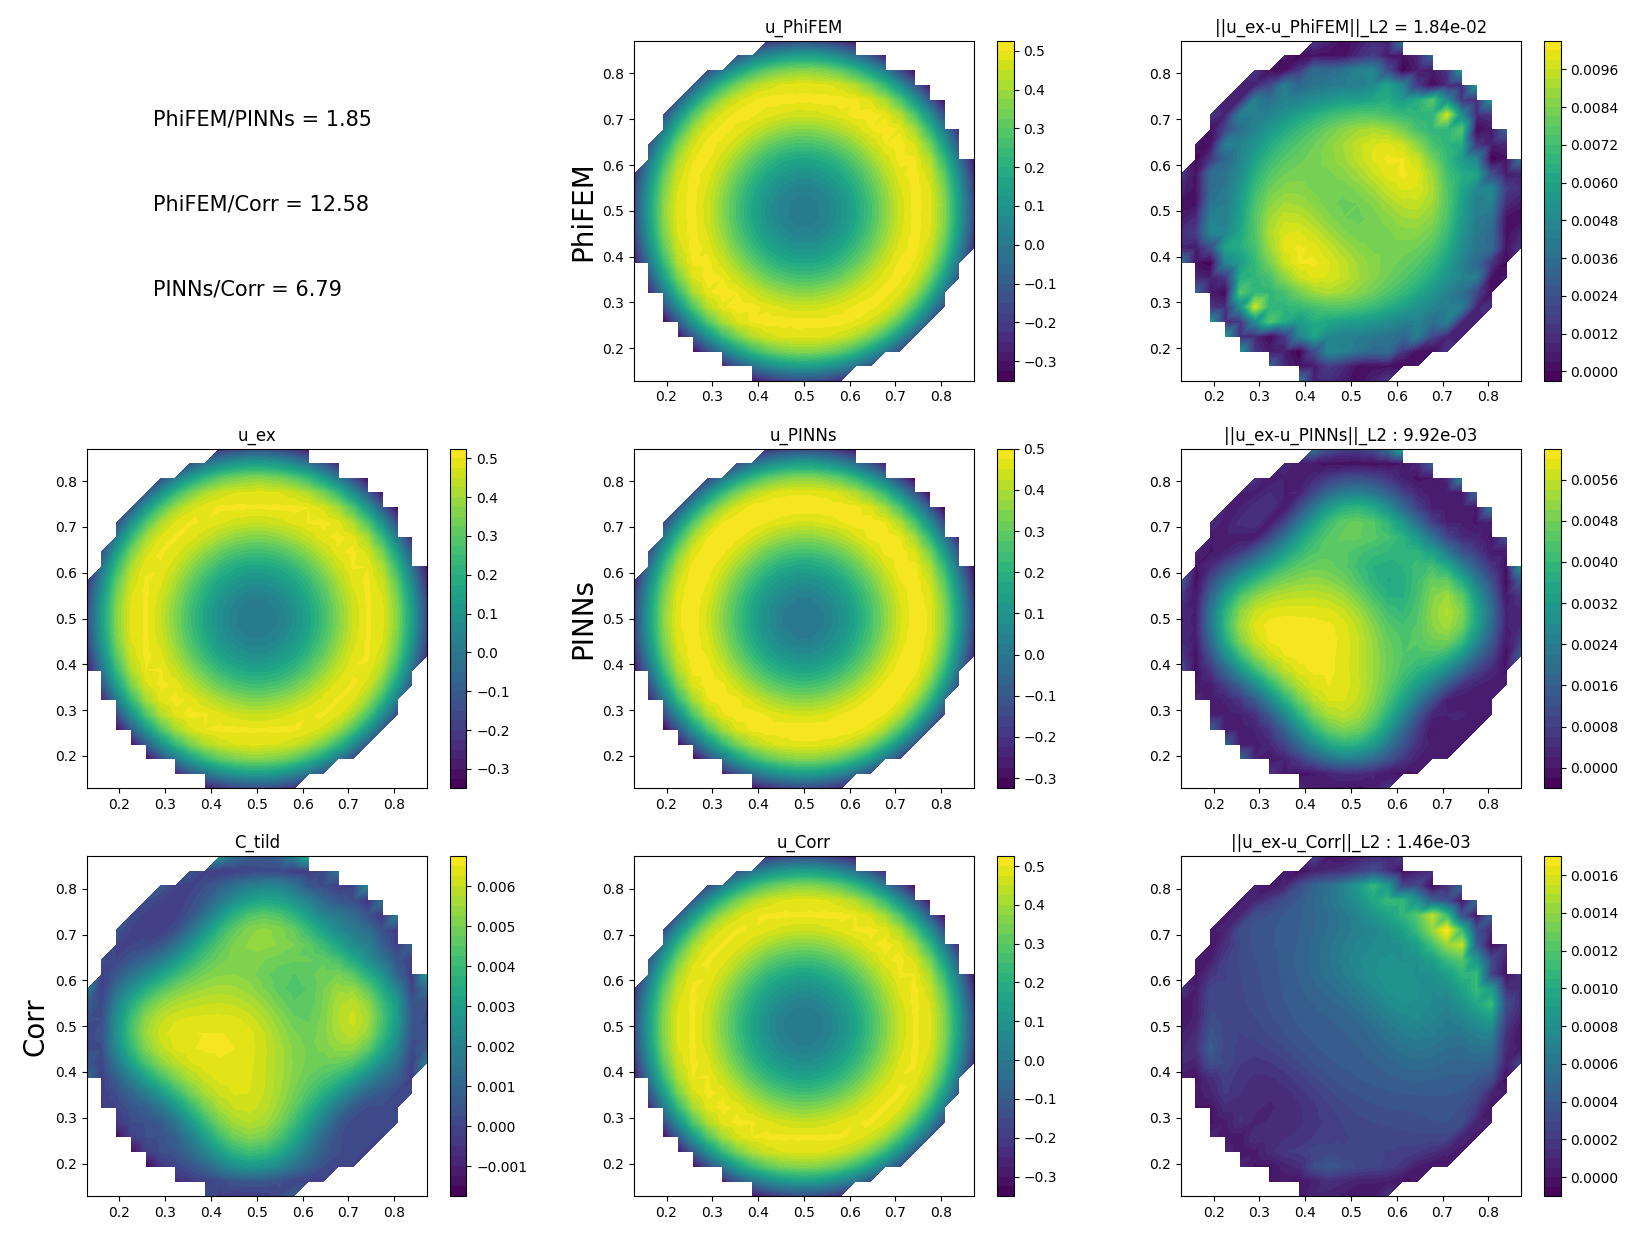
\includegraphics[width=\linewidth]{"varier_f/Poisson2D_fixed_corr_phifem_0_exact_bc.png"}
		\caption{Correction avec $\phi$-FEM - $f$ fixé.}
	\end{figure}
\end{minipage}
\begin{minipage}{0.48\linewidth}
	\begin{figure}[H]
		\centering
		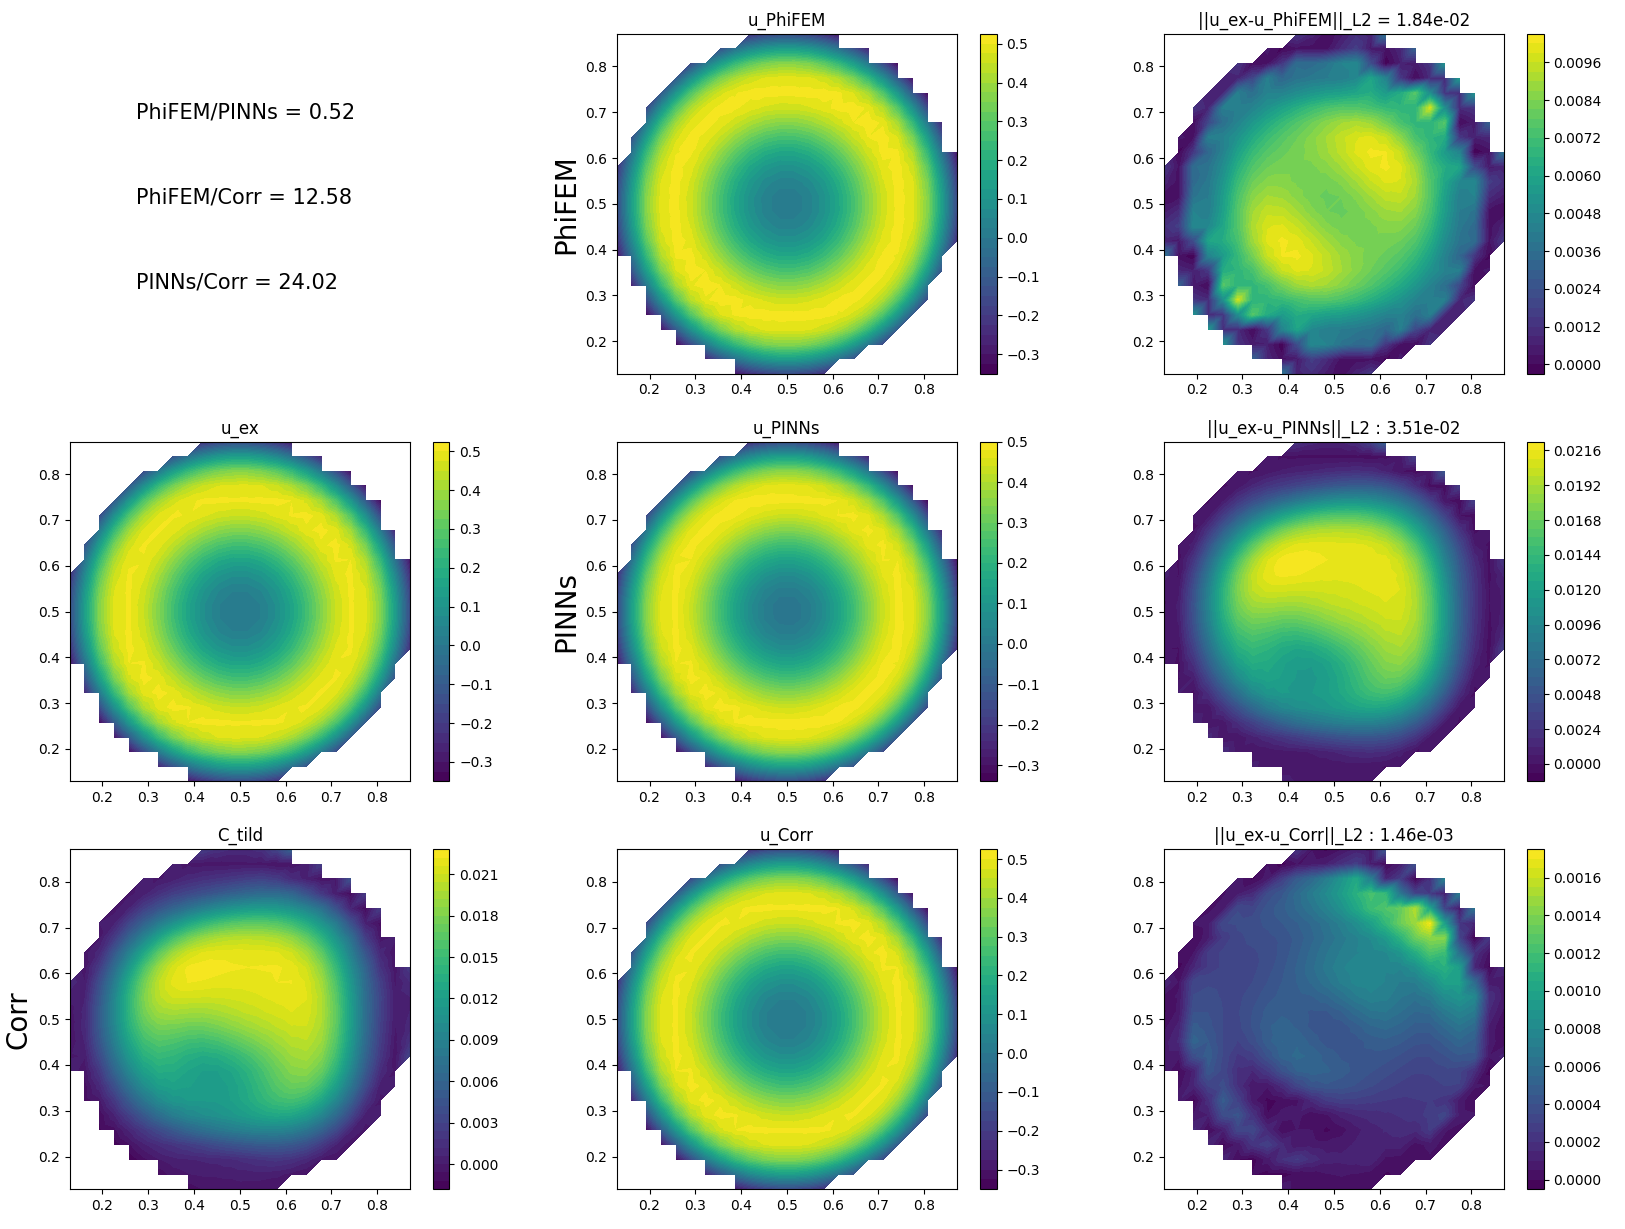
\includegraphics[width=\linewidth]{"varier_f/Poisson2D_f_corr_phifem_0_exact_bc.png"}
		\caption{Correction avec $\phi$-FEM - $f$ qui varie.}
	\end{figure}
\end{minipage}

\begin{Obs}
	Cas $f$ qui varie :
	\begin{itemize}
		\item PINNs $\searrow$ (moins bon que FEM standard)
		\item correction avec $\phi$-FEM sur la prédiction $\nearrow$ 
		\item précision finale en comparaison de FEM standard $=$ (peut être due au fait que seul $S$ varie ? $\Rightarrow$ tester ajout de nouveaux paramètres dans l'entraînement comme la fréquence)
	\end{itemize}
\end{Obs}

